\chapter{DESAIN DAN IMPLEMENTASI}
\label{chap:desainimplementasi}


\section{Struktur Rencana Kerja Pengembangan (WBS)}
\sloppy
Penelitian ini menggunakan pendekatan pengembangan berbasis \emph{Work Breakdown Structure} (WBS), yaitu metode sistematis untuk membagi keseluruhan proses pengembangan ke dalam unit-unit kerja yang lebih kecil dan terstruktur. WBS mencakup tahapan analisis kebutuhan, perancangan, implementasi, hingga evaluasi, yang disusun secara hierarkis untuk memudahkan perencanaan dan pelaksanaan sistem secara efisien. Diagram WBS yang digunakan dalam penelitian ini dapat dilihat pada Gambar \ref{fig:wbs}.

\begin{figure}[H]
  \centering
  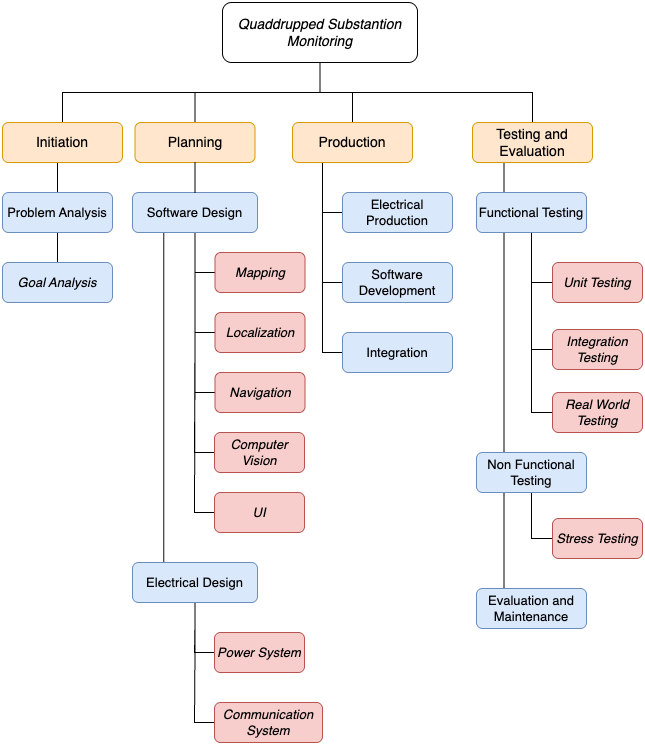
\includegraphics[width=0.8\textwidth]{gambar/bab3/wbs.png}
  \caption{\emph{Work Breakdown Structure} (WBS) Penelitian}
  \label{fig:wbs}
  \footnotesize{\textbf{Sumber:} Dokumentasi Pribadi}
\end{figure}

\section{Analisis Kebutuhan}
Analisis kebutuhan dilakukan melalui pengumpulan data dari studi literatur dan wawancara dengan pihak-pihak terkait. Berdasarkan hasil analisis. Adapun spesifikasi kebutuhan sistem yang harus dipenuhi dalam penelitian ini adalah sebagai berikut:

\newpage



\section{Perancangan Sistem (\emph{Planning})}

Desain elektrikal robot mencakup perancangan sistem distribusi daya dan komunikasi yang bertujuan untuk mengintegrasikan komponen-komponen tambahan ke dalam sistem robot yang sudah ada. Komponen-komponen tambahan tersebut dirancang untuk mendukung kemampuan operasi otonom robot. Desain elektrikal lengkap dari robot ini dapat dilihat pada Gambar \ref{fig:electrical}.

\begin{figure}[H]
  \centering
  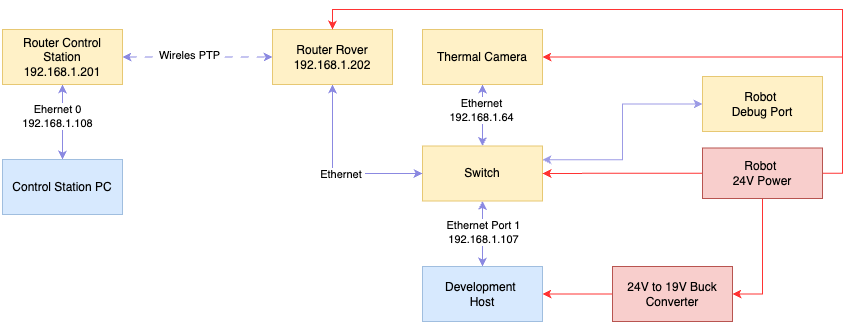
\includegraphics[width=0.9\textwidth]{gambar/bab3/electrical.png}
  \caption{Desain Elektrikal Robot}
  \label{fig:electrical}
  \footnotesize{\textbf{Sumber:} Dokumentasi Pribadi}
\end{figure}

\subsection{Integrasi Pengendalian dan Penghindaran}

Dalam sistem navigasi jalur otonom, integrasi antara pengendalian lintasan dan penghindaran rintangan menjadi sangat penting. Salah satu strategi umum adalah memanfaatkan PID atau Pure Pursuit sebagai pengendali utama lintasan, dan mengaktifkan modul penghindaran Braitenberg secara kondisional ketika objek terdeteksi pada jarak tertentu. Pendekatan ini memungkinkan sistem untuk tetap mengikuti jalur yang diinginkan, namun secara dinamis menghindari rintangan tanpa perlu perencanaan ulang jalur penuh.

Integrasi semacam ini dapat direalisasikan melalui skema \emph{behavior-based arbitration} atau \emph{subsumption architecture}, di mana penghindaran rintangan memiliki prioritas lebih tinggi saat kondisi kritis terdeteksi, kemudian dikembalikan ke kontrol jalur utama setelah lingkungan aman. Dengan demikian, sistem navigasi menjadi lebih adaptif, aman, dan efisien dalam lingkungan nyata yang dinamis.